\frame
{
\frametitle{Monitoreo y Control de Riesgos}

\begin{block}{}
Monitorear y controlar los riesgos es el proceso de \textbf{ejecución de planes} de respuesta ante el riesgo, el \textbf{seguimiento} de los riesgos identificados, \textbf{supervisar} los riesgos residuales, \textbf{identificando} nuevos riesgos, y \textbf{evaluar} la eficacia proceso de riesgo en todo el proyecto.
\end{block}

}

\frame
{
\frametitle{Monitoreo y Control de Riesgos}
\framesubtitle{Entradas}
\begin{columns}
	\begin{column}{0.8\textwidth}
		\begin{itemize}
			\item <1-> \textbf{Registro} de Riesgos
			\item <2-> \textbf{Plan} de Administración de Proyectos
			\item <3-> \textbf{Información} de Rendimiento en el Trabajo
			\item <4-> \textbf{Reportes} de Rendimiento
		\end{itemize}
	\end{column}
	\begin{column}{0.2\textwidth}
		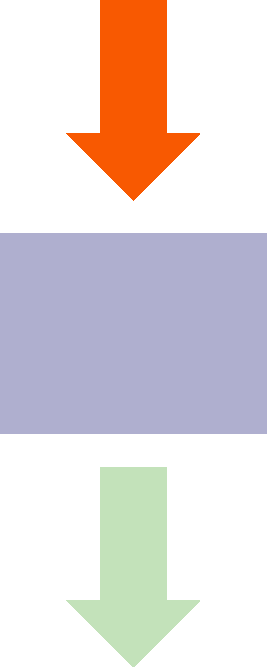
\includegraphics[width=2cm]{img/input}
	\end{column}
\end{columns}
}

\frame
{
\frametitle{Monitoreo y Control de Riesgos}
\framesubtitle{Herramientas y Técnicas}
\begin{columns}
	\begin{column}{0.8\textwidth}
		\begin{itemize}
			\item <1-> \textbf{Revaloración} de Riesgos
			\item <2-> \textbf{Auditorías} de Riesgos.
			\item <3-> \textbf{Varianza y Análisis} de Tendencias.
			\item <4-> \textbf{Medición} de Rendimiento Técnico
			\item <5-> \textbf{Análisis} de Reserva.
			\item <6-> \textbf{Reuniones} de Estado
		\end{itemize}
	\end{column}
	\begin{column}{0.2\textwidth}
		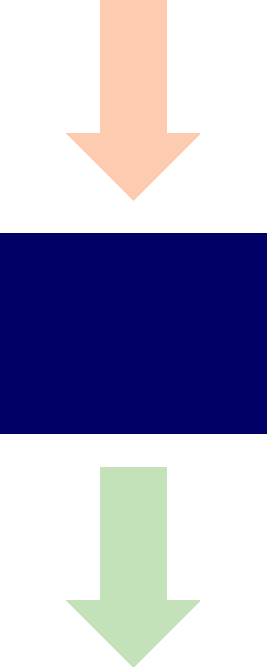
\includegraphics[width=2cm]{img/tools}
	\end{column}
\end{columns}
}

\frame
{
\frametitle{Monitoreo y Control de Riesgos}
\framesubtitle{Salidas}
\begin{columns}
	\begin{column}{0.8\textwidth}
		\begin{itemize}
			\item <1-> Actualizaciones de \textbf{Registro de Riesgos}
			\item <2-> Actualizaciones de los \textbf{Activos de Proceso de Organización}
			\item <3-> Solicitudes de \textbf{Cambio}
			\item <4-> Actualizaciones al \textbf{Plan de Administración de Proyecto}
			\item <5-> Actualizaciones al \textbf{Documento de Proyecto}
		\end{itemize}
	\end{column}
	\begin{column}{0.2\textwidth}
		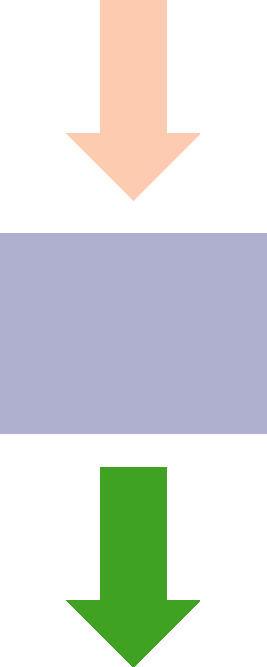
\includegraphics[width=2cm]{img/output}
	\end{column}
\end{columns}

}
